\documentclass[oneside,10pt]{book}

\usepackage{cdtBook}
\usepackage{usecases}

%Espacios
\newcommand\tab[1][1cm]{\hspace*{#1}}

\title{Análisis del sistema para la Liga de fútbol: El bolillo de ESCOM }
\subtitle{}
\author{Autores: \\Aguilera Ramírez Rubén Omar \\ Altamirano Lara Jesús David \\ Arredondo Basurto Edgar Rodrigo \\ Fernández Quiñones Isaac \\ Flores Mejía Irving Alan \\ Galicia Vargas Gerardo \\ Hernández Gómez Ricardo Neftali \\ Hernández Quintero Victor \\ Landa Aguirre Rafael\\ Morales García Miguel Ángel \\ Mundo López Alejandro Edgar \\ \\}
\organization{Escuela Superior de Cómputo, IPN}

%%%%%%%%%%%%%%%%%%%%%%%%%%%%%%%%%%%%%%%%%%%%%%%%%%%%%%%%%%%%%%%%
\begin{document}

\maketitle
\thispagestyle{empty}

\frontmatter
\tableofcontents

\mainmatter

%=========================================================
\chapter{Introducción}

\cfinput{Introduccion}

%=========================================================
\chapter{Descripción del módulo de Torneos}

\cfinput{Descripcion}

%=========================================================
\chapter{Modelo de Negocios}
\begin{figure}[htbp!]
	\centering
		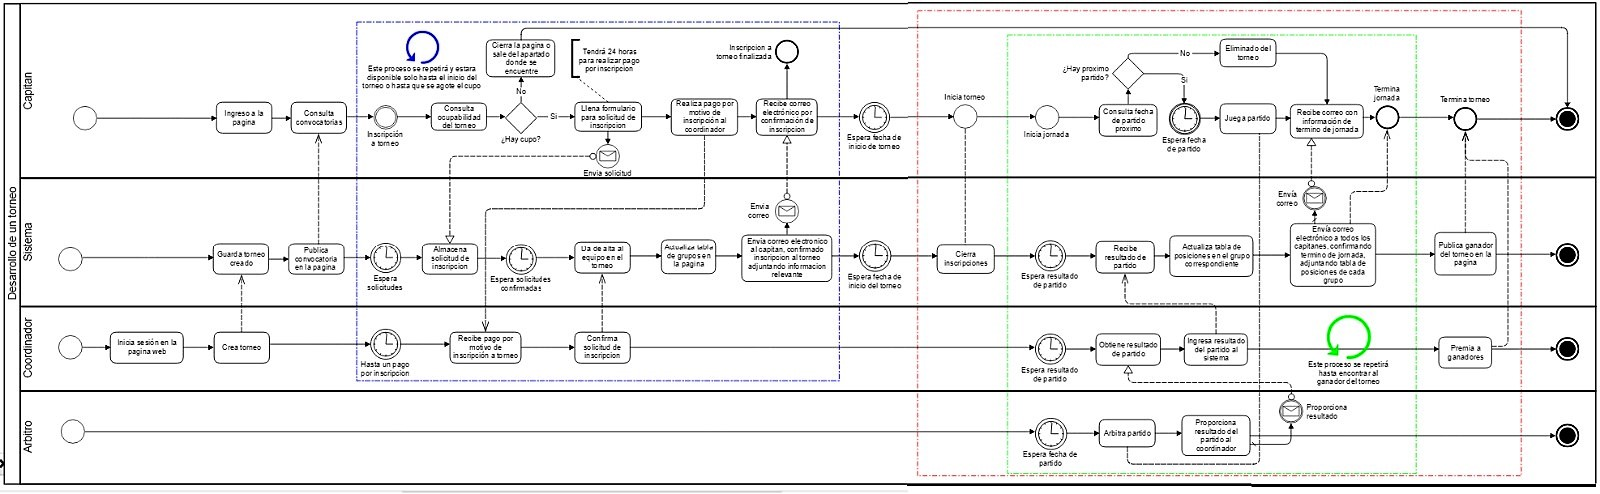
\includegraphics[width=.99\textwidth]{images/proceso}
	\caption{Diagrama de Proceso de Negocio.}
\end{figure}

%=========================================================
\chapter{Diagramas de Casos de uso}

\begin{figure}[htbp!]
	\centering
		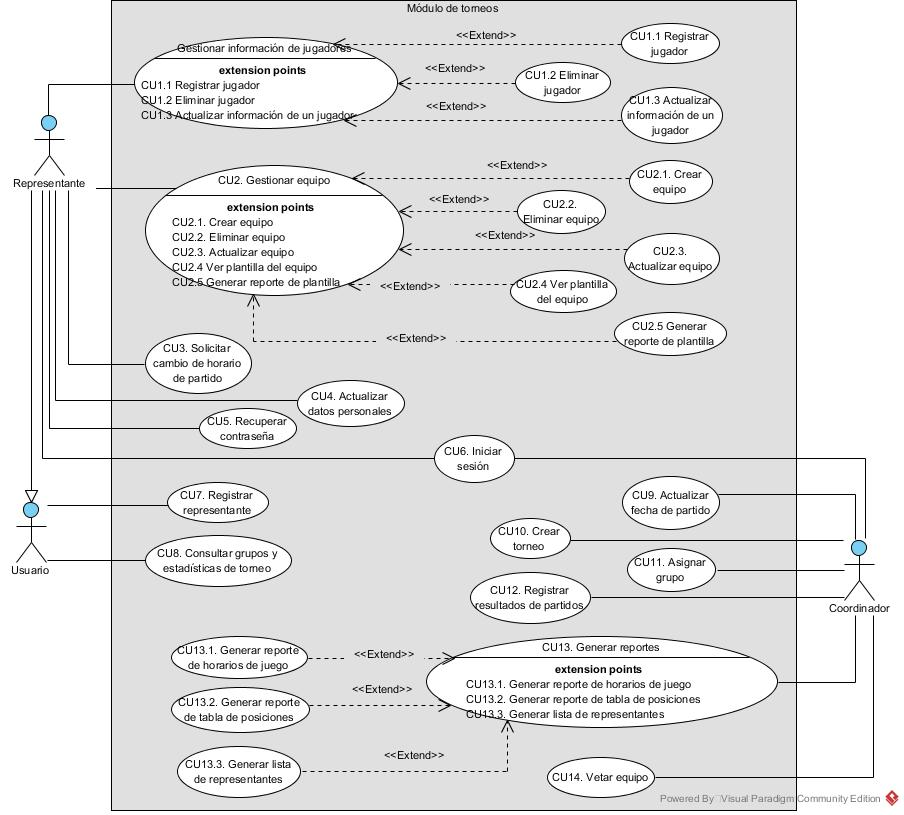
\includegraphics[width=.9\textwidth]{images/Torneo_Futbol}
	\caption{Diagrama de Casos de Uso del sistema.}
\end{figure}

%=========================================================
\chapter{Requisitos de software}

\cfinput{RF/requisitosFuncionales}

%=========================================================
\chapter{Actores}

\cfinput{Actores/Actores}

%=========================================================
\chapter{Modelo de Casos de Uso}

\cfinput{cu/CU1}
\cfinput{cu/CU1_1}
\cfinput{cu/CU1_2}
\cfinput{cu/CU1_3}
\cfinput{cu/CU2}
\cfinput{cu/CU2_1}
\cfinput{cu/CU2_2}
\cfinput{cu/CU2_3}
\cfinput{cu/CU2_4}
\cfinput{cu/CU2_5}
\cfinput{cu/CU3}
\cfinput{cu/CU4}
\cfinput{cu/CU5}
\cfinput{cu/CU6}
\cfinput{cu/CU7}
\cfinput{cu/CU8}
\cfinput{cu/CU9}
\cfinput{cu/CU10}
\cfinput{cu/CU11}
\cfinput{cu/CU12}
\cfinput{cu/CU13}
\cfinput{cu/CU13_1}
\cfinput{cu/CU13_2}
\cfinput{cu/CU13_3}
\cfinput{cu/CU14}

%%=========================================================
\chapter{Modelo de la Interacción}

{\color{UCInterfaceColor} 
	Esta sección se queda deliberadamente en blanco debido a que el diseño de las interfaces dependerá de la plataforma a utilizar por cada equipo.\\	
}

\cfinput{Pantallas/IU0}
\cfinput{Pantallas/IU1_0}
\cfinput{Pantallas/IU1_1}
\cfinput{Pantallas/IU1_2}
\cfinput{Pantallas/IU1_3}
\cfinput{Pantallas/IU2_1}
\cfinput{Pantallas/IU2_2}
\cfinput{Pantallas/IU2_3}
\cfinput{Pantallas/IU2_4}
\cfinput{Pantallas/IU2_5}
\cfinput{Pantallas/IU3_0}
\cfinput{Pantallas/IU4_0}
\cfinput{Pantallas/IU5_0}
\cfinput{Pantallas/IU6}
\cfinput{Pantallas/IU7}
\cfinput{Pantallas/IU8}
\cfinput{Pantallas/IU10}
\cfinput{Pantallas/IU10_1}
\cfinput{Pantallas/IU11}
%%=========================================================
\chapter{Glosario de términos}

\cfinput{reglas}

\end{document}

